% Copyright 2019 Clara Eleonore Pavillet

% Author: Clara Eleonore Pavillet
% Description: This is an unofficial Oxford University Beamer Template I made from scratch. Feel free to use it, modify it, share it.
% Version: 1.0

\documentclass{beamer}
% Load Packages
\usepackage[utf8]{inputenc}
\usepackage{xcolor}
\usepackage{tikz}
\usetikzlibrary{positioning,calc}
\usepackage{graphicx}
\usepackage{hyperref}
\usepackage{amsmath}
\usepackage{listings}
\usepackage{fontawesome}

% Define Commands
\newcommand*{\ClipSep}{0.06cm} %To adjust footer logo
\newcommand{\E}{\mathrm{e}\,} %\def\I{e} % used to defined e for exp(x), see later what it should be
\newcommand{\ud}{\mathrm{d}}
\lstset{numbers=left, numberstyle=\tiny, stepnumber=1,firstnumber=1,breaklines=true,
    numbersep=5pt,language=Python,
    stringstyle=\ttfamily,
    basicstyle=\footnotesize, 
    showstringspaces=false
}

\usetheme{oxonian}

\title{Gaussian Naive Bayes Classifier: Iris Data Set}
\titlegraphic{
\includegraphics[width=2cm]{Theme/Logos/logoTDTU.png}}
\author{Nguyen Van Hai \break Nguyen Tien Dung \break Dao Anh Huy \break Luu Thanh Duy}
\institute{Ton Duc Thang University}
\date{} %\today

\begin{document}

{\setbeamertemplate{footline}{} 
\frame{\titlepage}}

\section*{Outline}
    \begin{frame}{Outline}
        Overview \\
            \hspace{1cm} Iris Data Set \\
            \hspace{1cm} Bayes Theorem \\
            \hspace{1cm} Normal distribution \\
        Prepare Data \\
            \hspace{1cm} Load Data \\
            \hspace{1cm} Split Data \\
            \hspace{1cm} Group Data \\
        Summarize Data \\
            \hspace{1cm} Mean \\
            \hspace{1cm} Standard Deviation \\
            \hspace{1cm} Summary \\
    \end{frame}

    \begin{frame}{Outline}
        Build Model \\
            \hspace{1cm} Overview \\
            \hspace{1cm} Prior Probability \\
            \hspace{1cm} Likelihood \\
            \hspace{1cm} Joint Probability \\
            \hspace{1cm} Marginal Probability \\
            \hspace{1cm} Posterior Probability \\
        Test Model \\
            \hspace{1cm} Get Maximum A Posterior \\
            \hspace{1cm} Predict \\
            \hspace{1cm} Accuracy \\
        Code \\
        Results \\
            \hspace{1cm}  Print the results\\
    \end{frame}

\section{Overview}
    \begin{frame}[plain]
        \vfill
      \centering
      \begin{beamercolorbox}[sep=8pt,center,shadow=true,rounded=true]{title}
        \usebeamerfont{title}\insertsectionhead\par%
        \color{oxfordblue}\noindent\rule{10cm}{1pt} \\
        \LARGE{\faFileTextO}
      \end{beamercolorbox}
      \vfill
  \end{frame}


\subsection{Iris Data Set}
    \begin{frame}{Iris Data Set}
        \hspace{0.5cm}The data set has 4 independent variables and 1 dependent variable that have 3 different classes with 150 instances. \break
         - The first 4 columns are the independent variables (features). \break
         - The 5th column is the dependent variable (class).
        \begin{enumerate}
            \item sepal length (cm)
            \item sepal width (cm)
            \item petal length (cm)
            \item petal width (cm)
            \item class:
            \begin{itemize}
                \item Iris Setosa
                \item Iris Versicolour
                \item Iris Virginica
            \end{itemize}
        \end{enumerate}
    \end{frame}

    \begin{frame}{Iris Data Set}
        \hspace{0.5cm}For example:
        \begin{center}
            \begin{figure}
                \begin{center}
                     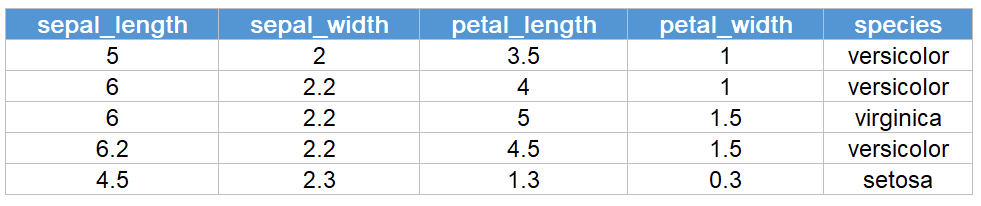
\includegraphics[width = 10cm, height = 3cm]{Theme/images/irisDataSet.png}
                \end{center}
                \caption{Random 5 Row Sample}
            \end{figure}
        \end{center}
    \end{frame}

\subsection{Bayes Theorem}
    \begin{frame}{Bayes Theorem}
        \hspace{0.5cm} Naive Bayes, more technically referred to as the Posterior Probability, updates the prior belief of an event given new information. The result is the probability of the class occuring given the new data.
        
        \begin{align*}
            P(class/features) = \frac{P(class) * P(features/class)}{P(features)}
        \end{align*}
        
        \begin{itemize}
            \item P(class/features) : Posterior Probability
            \item P(class) : Class Prior Probability
            \item P(features/class) : Likelihood
            \item P(features) : Predictor Prior Probability
        \end{itemize}
    \end{frame}

\subsection{Normal distribution}
    \begin{frame}{Normal distribution}
        \hspace{0.5cm} The probability density of the normal distribution is:
        \only{
        \begin{equation}
        f(x | \mu,\,\sigma^{2})=\frac{1}{\sqrt{2\,\pi \sigma^{2}}}\,\E^{-\frac{\left(x-\mu\right)^2}{2\,\sigma^2} }
        \end{equation}}
        \hspace{0.1cm}Where
        \begin{itemize}
            \item '${\mu}$' is the mean or expectation of the distribution, \\
            \item '${\sigma}$' is the standard deviation, and \\
            \item '${\sigma^2}$' is the variance. \\
        \end{itemize}
    \end{frame}


\section{Prepare Data}
    \begin{frame}[plain]
        \vfill
      \centering
      \begin{beamercolorbox}[sep=8pt,center,shadow=true,rounded=true]{title}
        \usebeamerfont{title}\insertsectionhead\par%
        \color{oxfordblue}\noindent\rule{10cm}{1pt} \\
        \LARGE{\faFileTextO}
      \end{beamercolorbox}
      \vfill
  \end{frame}
  
\subsection{Load Data}
    \begin{frame}{Load Data}
        \hspace{0.5cm} Read in the raw data and convert each string into an integer.
        \begin{center}
            \begin{figure}
                \begin{center}
                     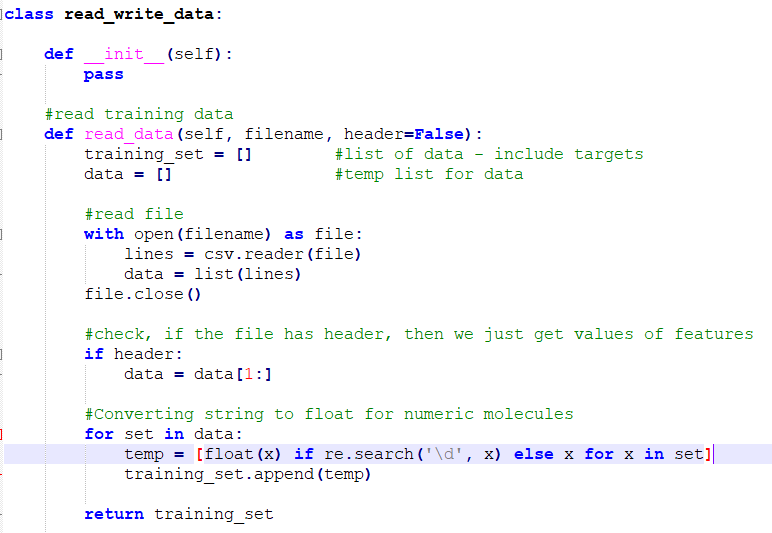
\includegraphics[width = 10cm, height = 7cm]{Theme/images/readData.PNG}
                \end{center}
            \end{figure}
        \end{center}
    \end{frame}

\subsection{Split Data}
    \begin{frame}{Split Data}
        \hspace{0.5cm} Split the data into a training\_set and a testing\_set. \\
        \hspace{0.5cm} The weight will determine how much of the data will be in the training\_set.
        \begin{center}
            \begin{figure}
                \begin{center}
                    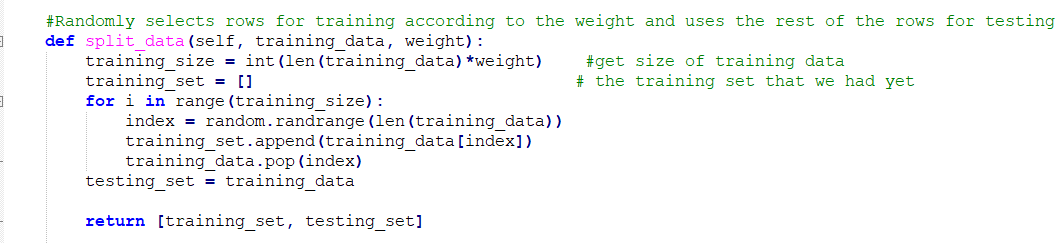
\includegraphics[width = 10cm, height = 3cm]{Theme/images/split.PNG}
                \end{center}
            \end{figure}
        \end{center}
    \end{frame}

\subsection{Group Data}
    \begin{frame}{Group Data}
        \hspace{0.5cm} Group the data according to class by mapping each class to individual instances.
        \begin{center}
            \begin{figure}
                \begin{center}
                    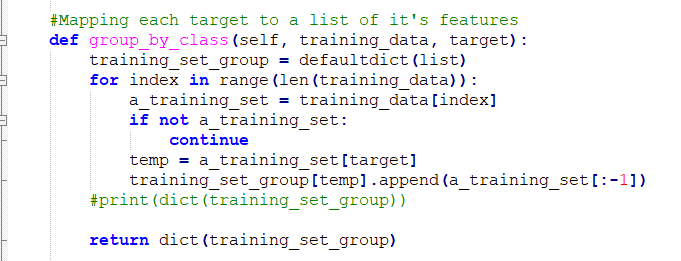
\includegraphics[width = 10cm, height = 5cm]{Theme/images/group.PNG}
                \end{center}
            \end{figure}
        \end{center}
    \end{frame}

\section{Summarize Data}
    \begin{frame}[plain]
        \vfill
      \centering
      \begin{beamercolorbox}[sep=8pt,center,shadow=true,rounded=true]{title}
        \usebeamerfont{title}\insertsectionhead\par%
        \color{oxfordblue}\noindent\rule{10cm}{1pt} \\
        \LARGE{\faFileTextO}
      \end{beamercolorbox}
      \vfill
  \end{frame}
  
\subsection{Mean}
    \begin{frame}{Mean}
        \hspace{0.5cm} Calculate the mean.
        \begin{center}
            \begin{figure}
                \begin{center}
                    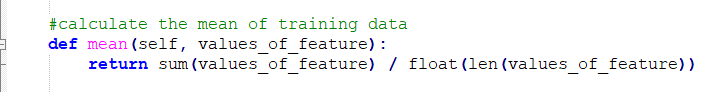
\includegraphics[width = 10cm, height = 2cm]{Theme/images/mean.PNG}
                \end{center}
            \end{figure}
        \end{center}
    \end{frame}

\subsection{Standard Deviation}
    \begin{frame}{Standard Deviation}
        \hspace{0.5cm} Calculate the standard deviation.
        \begin{center}
            \begin{figure}
                \begin{center}
                    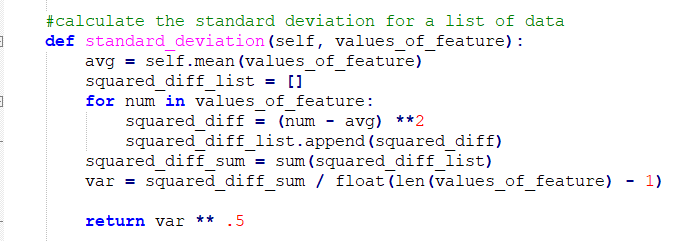
\includegraphics[width = 10cm, height = 5cm]{Theme/images/stdev.PNG}
                \end{center}
            \end{figure}
        \end{center}
    \end{frame}

\subsection{Summary}
    \begin{frame}{Summary}
        \hspace{0.5cm} Return the (mean, standard deviation) combination for each feature of the training\_set. The mean and the standard deviation will be used when calculating the Normal Probabiltiy values for each feature of the testing\_set.
        \begin{center}
            \begin{figure}
                \begin{center}
                    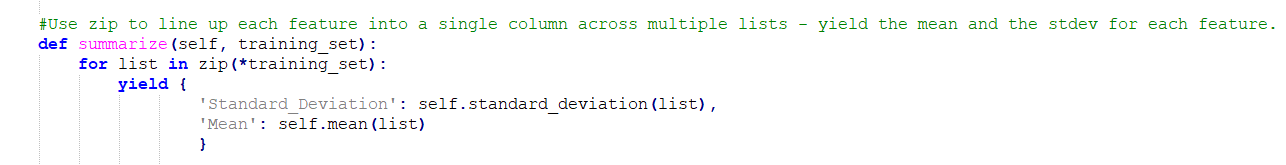
\includegraphics[width = 10cm, height = 3cm]{Theme/images/summary.PNG}
                \end{center}
            \end{figure}
        \end{center}
    \end{frame}

\section{Build Model}
    \begin{frame}[plain]
        \vfill
      \centering
      \begin{beamercolorbox}[sep=8pt,center,shadow=true,rounded=true]{title}
        \usebeamerfont{title}\insertsectionhead\par%
        \color{oxfordblue}\noindent\rule{10cm}{1pt} \\
        \LARGE{\faFileTextO}
      \end{beamercolorbox}
      \vfill
  \end{frame}
  
\subsection{Overview}
    \begin{frame}{Overview : Features and Class}
        \begin{center}
            \begin{figure}
                \begin{center}
                    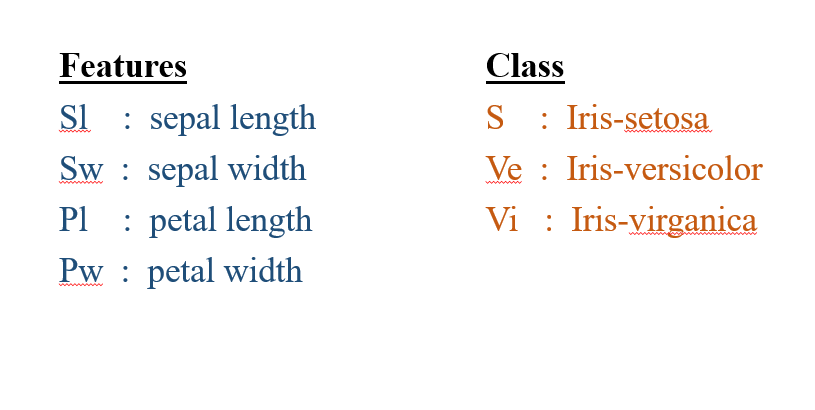
\includegraphics[width = 10cm, height = 5cm]{Theme/images/featuresAndClass.PNG}
                \end{center}
            \end{figure}
        \end{center}
    \end{frame}

\subsection{Overview}
    \begin{frame}{Overview : Bayes Tree Diagram}
        \begin{center}
            \begin{figure}
                \begin{center}
                    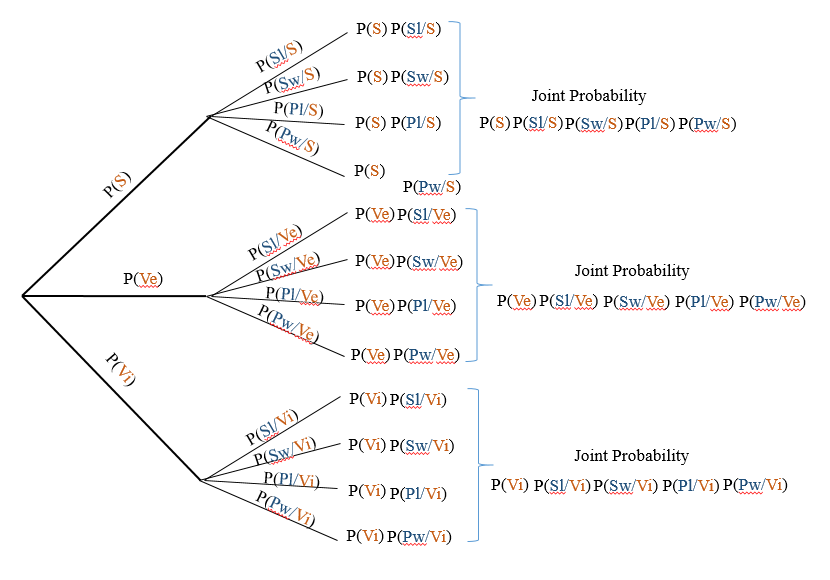
\includegraphics[width = 10cm, height = 7cm]{Theme/images/tree.PNG}
                \end{center}
            \end{figure}
        \end{center}
    \end{frame}

\subsection{Prior Probability}
    \begin{frame}{Prior Probability}
        \hspace{0.5cm} Prior Probability is what we know about each class before considering the new data. \\
        \hspace{0.5cm} It's the probability of each class occurring. \\
        \begin{center}
            \begin{figure}
                \begin{center}
                    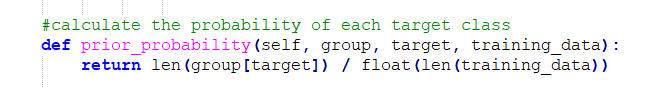
\includegraphics[width = 10cm, height = 2cm]{Theme/images/prior_prob.PNG}
                \end{center}
            \end{figure}
        \end{center}
    \end{frame}

\subsection{Train}
    \begin{frame}{Train}
        \hspace{0.5cm} This is where we learn from the train set, by calculating the mean and the standard deviation.\\
        \hspace{0.5cm} Using the grouped classes, calculate the (mean, standard deviation) combination for each feature of each class. \\
        \hspace{0.5cm} The calculations will later use the (mean, standard deviation) of each feature to calculate class likelihoods. \\
        \begin{center}
            \begin{figure}
                \begin{center}
                    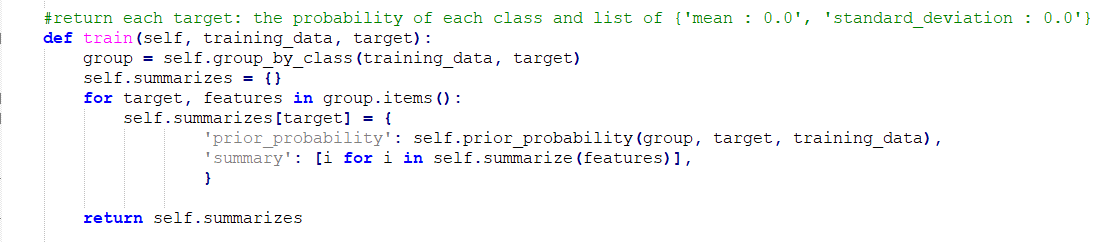
\includegraphics[width = 10cm, height = 4cm]{Theme/images/train.PNG}
                \end{center}
            \end{figure}
        \end{center}
    \end{frame}

\subsection{Likelihood}
    \begin{frame}{Likelihood}
        \hspace{0.5cm} Likelihood is calculated by taking the product of all Normal Probabilities. 
        \begin{center}
            \textcolor[rgb]{1.0,0.0,0.0} {P(features/class)}\\
        \end{center}
        \hspace{0.5cm} For each feature given the class we calculate the Normal Probability using the Normal Distribution. 
        \begin{center}
            \textcolor[rgb]{1.0,0.0,0.0}{P(Sl/S)P(Sw/S)P(Pl/S)P(Pw/S)}\\
        \end{center}
        \begin{center}
            \begin{figure}
                \begin{center}
                    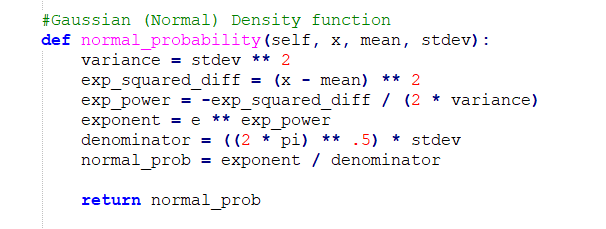
\includegraphics[width = 10cm, height = 4cm]{Theme/images/normal_probs.PNG}
                \end{center}
            \end{figure}
        \end{center}
    \end{frame}

\subsection{Joint Probability}
    \begin{frame}{Joint Probability}
        \hspace{0.5cm} Joint Probability is calculated by taking the product of the Prior Probability and the Likelihood.
        \begin{center}
            \textcolor[rgb]{1.0,0.0,0.0} {P(S)P(Sl/S)P(Sw/S)P(Pl/S)P(Pw/S)}\\
        \end{center}
        \begin{center}
            \begin{figure}
                \begin{center}
                     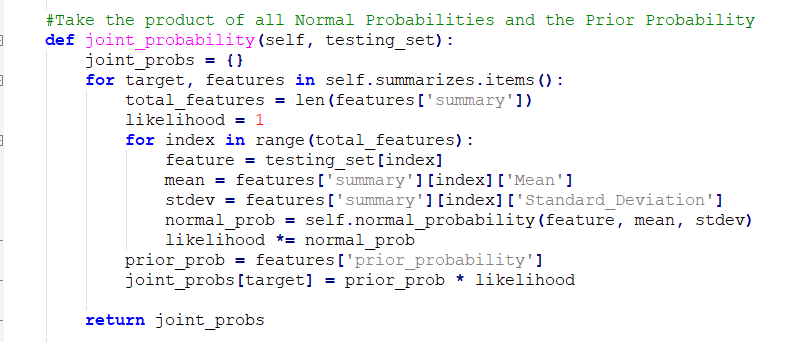
\includegraphics[width = 10cm, height = 5cm]{Theme/images/joint_probs.PNG}
                \end{center}
            \end{figure}
        \end{center}
    \end{frame}

\subsection{Marginal Probability}
    \begin{frame}{Marginal Probability}
        \hspace{0.5cm} Calculate the total sum of all joint probabilities.
        \begin{center}
            \textcolor[rgb]{1.0,0.0,0.0} {Marginal\_probs = P(S)P(Sl/S)P(Sw/S)P(Pl/S)P(Pw/S) 
                                                         + P(Ve)P(Sl/Ve)P(Sw/Ve)P(Pl/Ve)P(Pw/Ve) 
                                                         + P(Vi)P(Sl/Vi)P(Sw/Vi)P(Pl/Vi)P(Pw/Vi)}\\
        \end{center}
        \begin{center}
            \begin{figure}
                \begin{center}
                    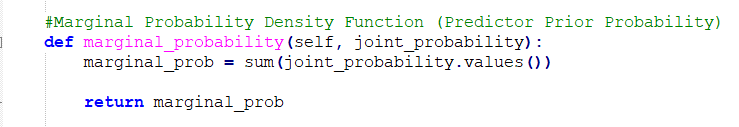
\includegraphics[width = 10cm, height = 3cm]{Theme/images/margimal_probs.PNG}
                \end{center}
            \end{figure}
        \end{center}
    \end{frame}

\subsection{Posterior Probability}
    \begin{frame}{Posterior Probability}
        \hspace{0.5cm} The Posterior Probability is the probability of a class occuring and is calculated for each class given the new data.
        \begin{center}
            \textcolor[rgb]{1.0,0.0,0.0} {P(class/features)}\\
        \end{center}
        \hspace{0.5cm} This where all of the preceding class methods tie together to calculate the Gauss Naive Bayes formula with the goal of selecting MAP. \\
        \begin{center}
            \begin{figure}
                \begin{center}
                    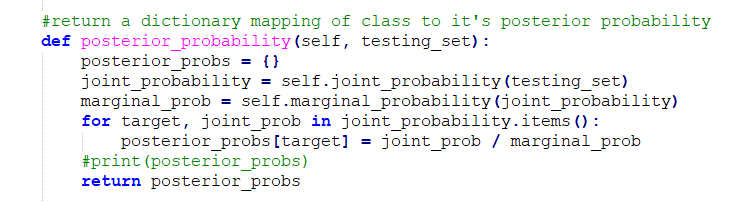
\includegraphics[width = 10cm, height = 4cm]{Theme/images/posterior_probs.PNG}
                \end{center}
            \end{figure}
        \end{center}
    \end{frame}

\section{Test Model}
    \begin{frame}[plain]
        \vfill
      \centering
      \begin{beamercolorbox}[sep=8pt,center,shadow=true,rounded=true]{title}
        \usebeamerfont{title}\insertsectionhead\par%
        \color{oxfordblue}\noindent\rule{10cm}{1pt} \\
        \LARGE{\faFileTextO}
      \end{beamercolorbox}
      \vfill
  \end{frame}
  
\subsection{Get Maximum A Posterior}
    \begin{frame}{Get Maximum A Posterior}
        \hspace{0.5cm} The get\_best\_posterior\_probability() method will call the posterior\_probability() method on a single test\_row. \\
        \hspace{0.5cm} For each test\_row we will calculate 3 Posterior Probabilities; one for each class. The goal is to select MAP, the Maximum A Posterior probability. \\
        \hspace{0.5cm} The get\_best\_posterior\_probability() method will simply choose the Maximum A Posterior probability and return the associated class for the given test\_row.\\
        \begin{center}
            \begin{figure}
                \begin{center}
                    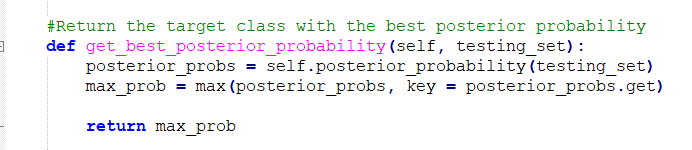
\includegraphics[width = 10cm, height = 3cm]{Theme/images/get_best.PNG}
                \end{center}
            \end{figure}
        \end{center}
    \end{frame}

\subsection{Predict}
    \begin{frame}{Predict}
        \hspace{0.5cm} This method will return a prediction for each test\_row. \\
        \begin{center}
            \begin{figure}
                \begin{center}
                    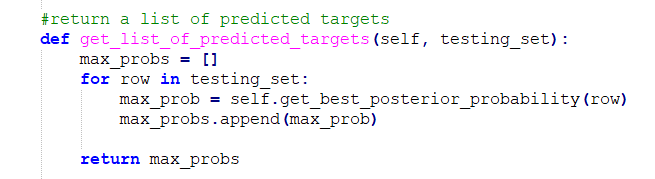
\includegraphics[width = 10cm, height = 3cm]{Theme/images/get_list.PNG}
                \end{center}
            \end{figure}
        \end{center}
    \end{frame}

\subsection{Accuracy}
    \begin{frame}{Accuracy}
    \hspace{0.5cm} Accuracy will test the performance of the model by taking the total number of correct predictions and divide them by the total number of predictions. This is critical in understanding the veracity of the model. \\
    \begin{center}
        \begin{figure}
            \begin{center}
                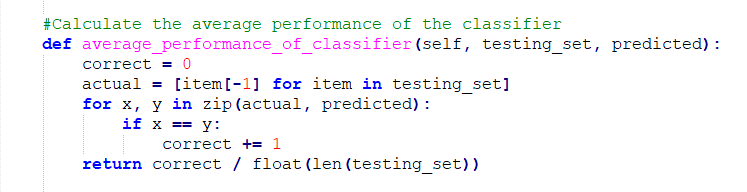
\includegraphics[width = 10cm, height = 4cm]{Theme/images/average.PNG}
            \end{center}
        \end{figure}
    \end{center}
    \end{frame}

\section{Code}
    \begin{frame}[plain]
        \vfill
      \centering
      \begin{beamercolorbox}[sep=8pt,center,shadow=true,rounded=true]{title}
        \usebeamerfont{title}\insertsectionhead\par%
        \color{oxfordblue}\noindent\rule{10cm}{1pt} \\
        \LARGE{\faFileTextO}
      \end{beamercolorbox}
      \vfill
  \end{frame}

\subsection{Code}
    \begin{frame}{Code}
        \begin{center}
            \begin{figure}
                \begin{center}
                     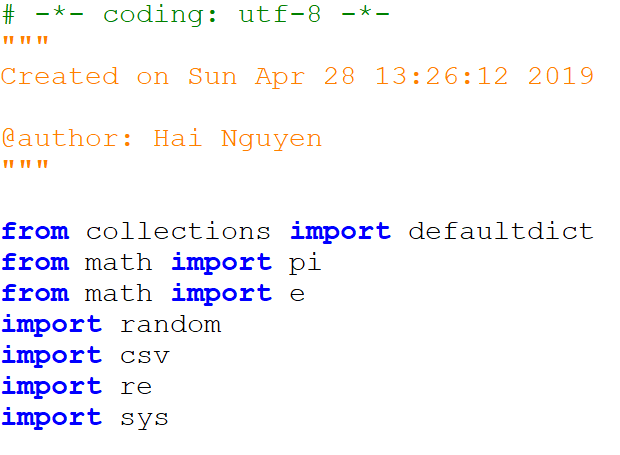
\includegraphics[width = 10cm, height = 5cm]{Theme/images/imports.PNG}
                \end{center}
            \end{figure}
        \end{center}
    \end{frame}

\subsection{Code}
    \begin{frame}{Code}
        \begin{center}
            \begin{figure}
                \begin{center}
                    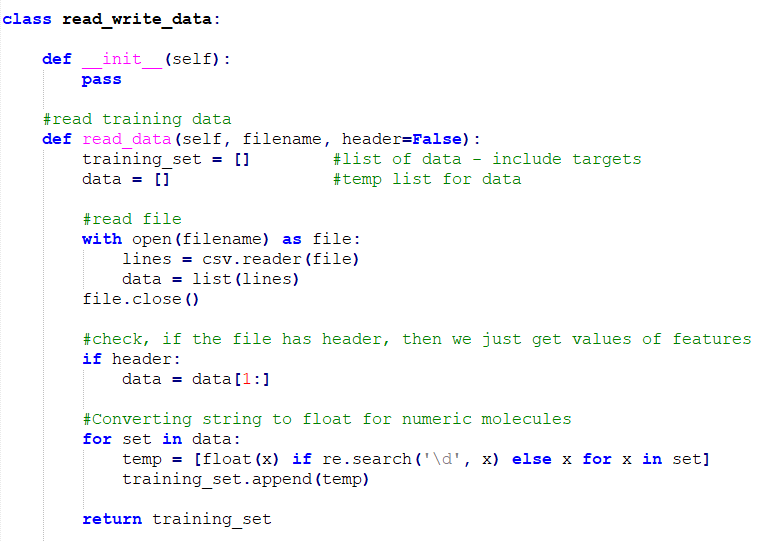
\includegraphics[width = 10cm, height = 6cm]{Theme/images/read.PNG}
                \end{center}
            \end{figure}
        \end{center}
    \end{frame}

\subsection{Code}
    \begin{frame}{Code}
        \begin{center}
            \begin{figure}
                \begin{center}
                    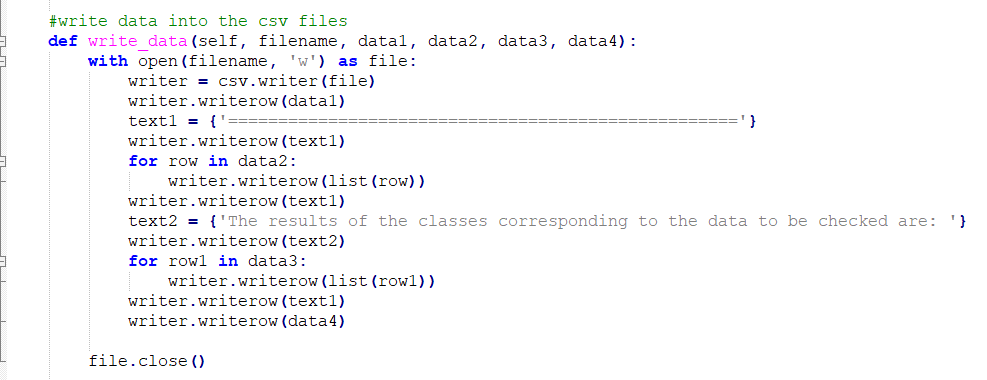
\includegraphics[width = 10cm, height = 5cm]{Theme/images/write.PNG}
                \end{center}
            \end{figure}
        \end{center}
    \end{frame}

\subsection{Code}
    \begin{frame}{Code}
        \begin{center}
            \begin{figure}
                \begin{center}
                     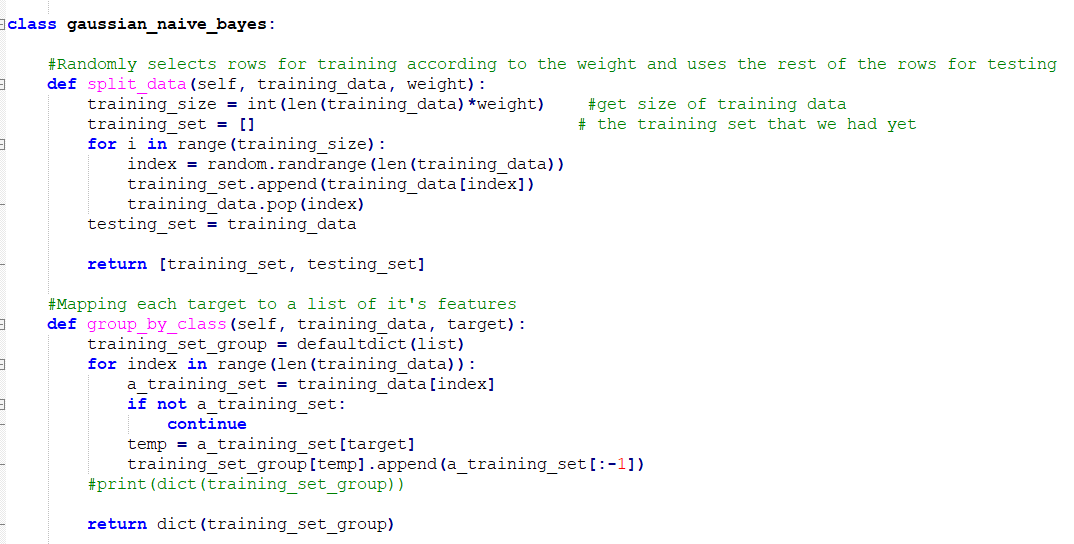
\includegraphics[width = 10cm, height = 7cm]{Theme/images/gaussian1.PNG}
                \end{center}
            \end{figure}
        \end{center}
    \end{frame}

\subsection{Code}
    \begin{frame}{Code}
        \begin{center}
            \begin{figure}
                \begin{center}
                    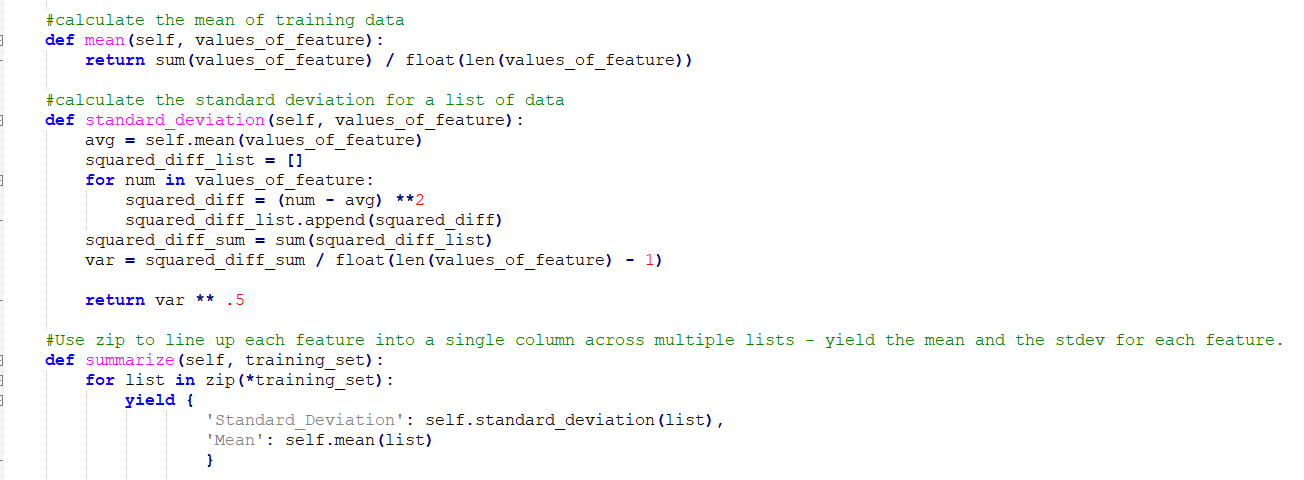
\includegraphics[width = 10cm, height = 7cm]{Theme/images/gaussian2.PNG}
                \end{center}
            \end{figure}
        \end{center}
    \end{frame}

\subsection{Code}
    \begin{frame}{Code}
        \begin{center}
            \begin{figure}
                \begin{center}
                    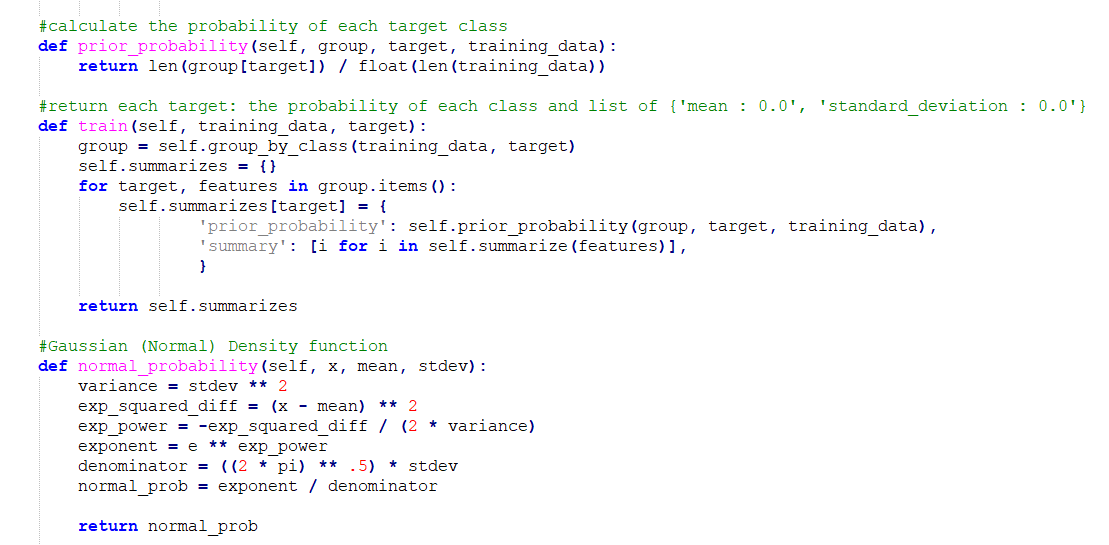
\includegraphics[width = 10cm, height = 7cm]{Theme/images/gaussian3.PNG}
                \end{center}
            \end{figure}
        \end{center}
    \end{frame}

\subsection{Code}
    \begin{frame}{Code}
        \begin{center}
            \begin{figure}
                \begin{center}
                    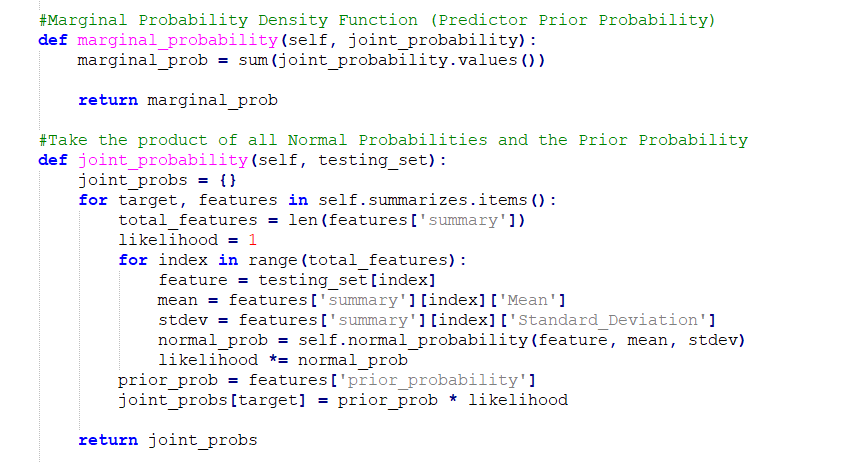
\includegraphics[width = 10cm, height = 7cm]{Theme/images/gaussian4.PNG}
                \end{center}
            \end{figure}
        \end{center}
    \end{frame}

\subsection{Code}
    \begin{frame}{Code}
        \begin{center}
            \begin{figure}
                \begin{center}
                    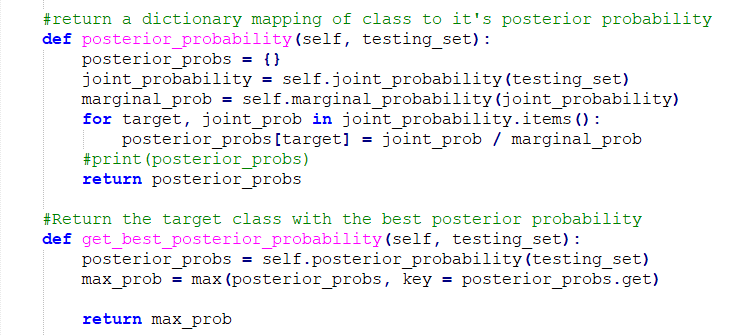
\includegraphics[width = 10cm, height = 5cm]{Theme/images/gaussian5.PNG}
                \end{center}
            \end{figure}
        \end{center}
    \end{frame}

\subsection{Code}
    \begin{frame}{Code}
        \begin{center}
            \begin{figure}
                \begin{center}
                     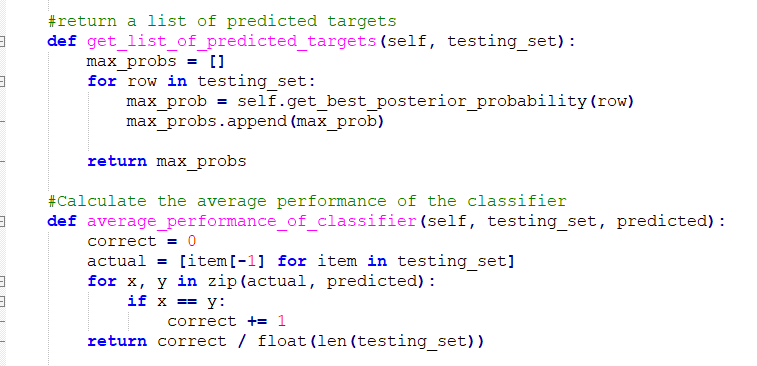
\includegraphics[width = 10cm, height = 5cm]{Theme/images/gaussian6.PNG}
                \end{center}
            \end{figure}
        \end{center}
    \end{frame}

\subsection{Code}
    \begin{frame}{Code}
        \begin{center}
            \begin{figure}
                \begin{center}
                    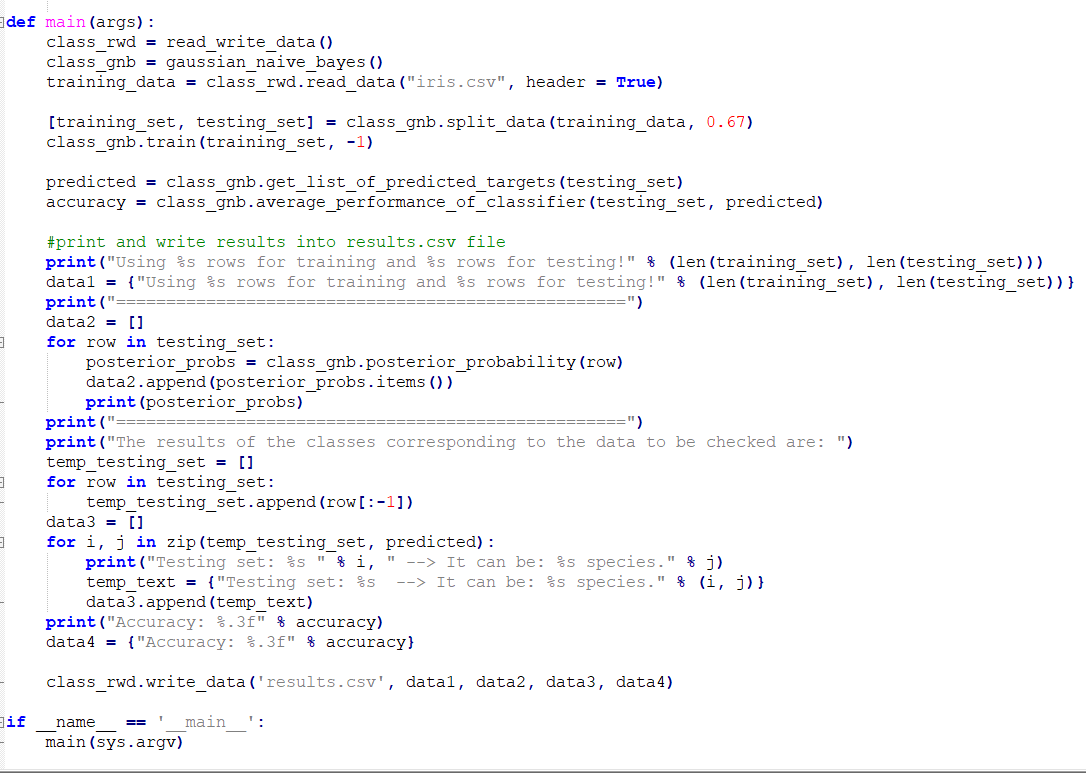
\includegraphics[width = 10cm, height = 7cm]{Theme/images/mains.PNG}
                \end{center}
            \end{figure}
        \end{center}
    \end{frame}

\section{Results}
    \begin{frame}[plain]
        \vfill
      \centering
      \begin{beamercolorbox}[sep=8pt,center,shadow=true,rounded=true]{title}
        \usebeamerfont{title}\insertsectionhead\par%
        \color{oxfordblue}\noindent\rule{10cm}{1pt} \\
        \LARGE{\faFileTextO}
      \end{beamercolorbox}
      \vfill
  \end{frame}

\subsection{Print the results}
    \begin{frame}{Print the results}
        \begin{center}
            \begin{figure}
                \begin{center}
                     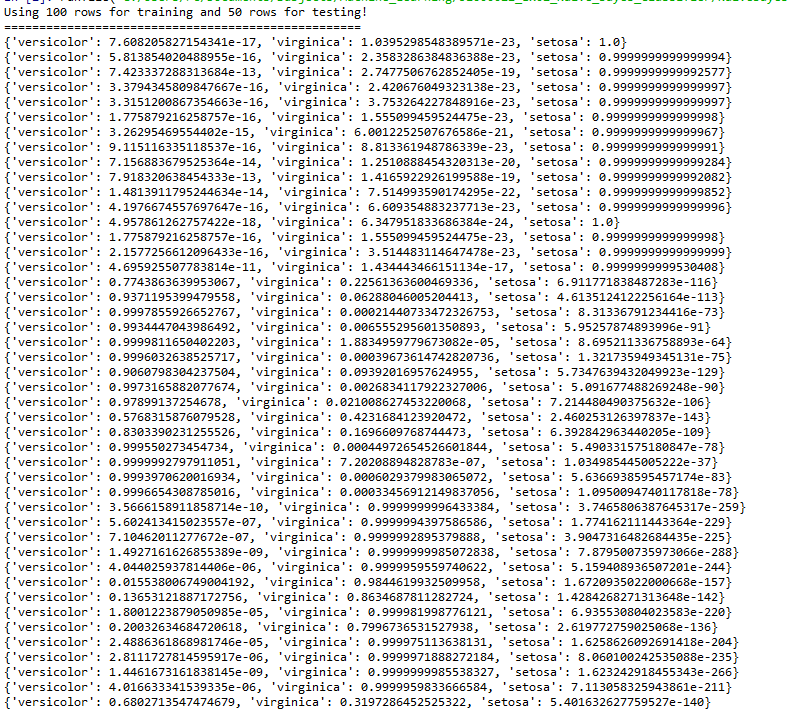
\includegraphics[width = 10cm, height = 7cm]{Theme/images/results1.PNG}
                \end{center}
            \end{figure}
        \end{center}
    \end{frame}

\subsection{Print the results}
    \begin{frame}{Print the results}
        \begin{center}
            \begin{figure}
                \begin{center}
                     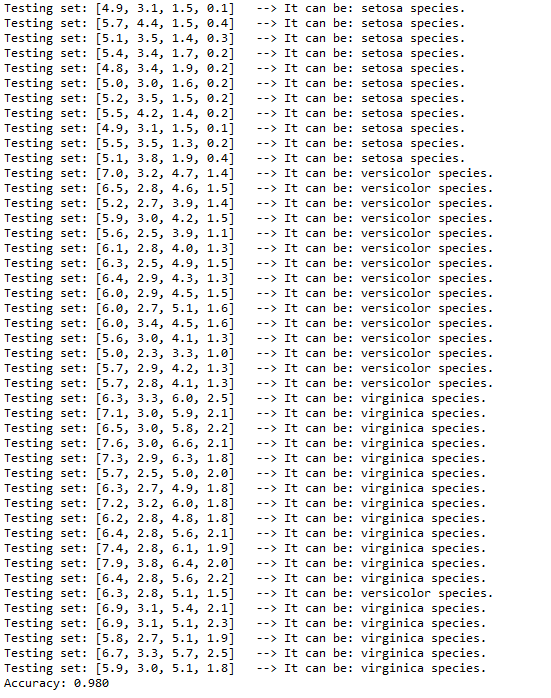
\includegraphics[width = 10cm, height = 7cm]{Theme/images/results2.PNG}
                \end{center}
            \end{figure}
        \end{center}
    \end{frame}

\section{THE END}
    \begin{frame}[plain]
        \vfill
      \centering
      \begin{beamercolorbox}[sep=8pt,center,shadow=true,rounded=true]{title}
        \usebeamerfont{title}\insertsectionhead\par%
        \color{oxfordblue}\noindent\rule{2cm}{1pt} \\
      \end{beamercolorbox}
      \vfill
  \end{frame}
\end{document}

